\section{Eclipse Modeling Framework}
\label{sec:background:eclipse_modeling_framework}

\begin{figure}[p]
    \centering
    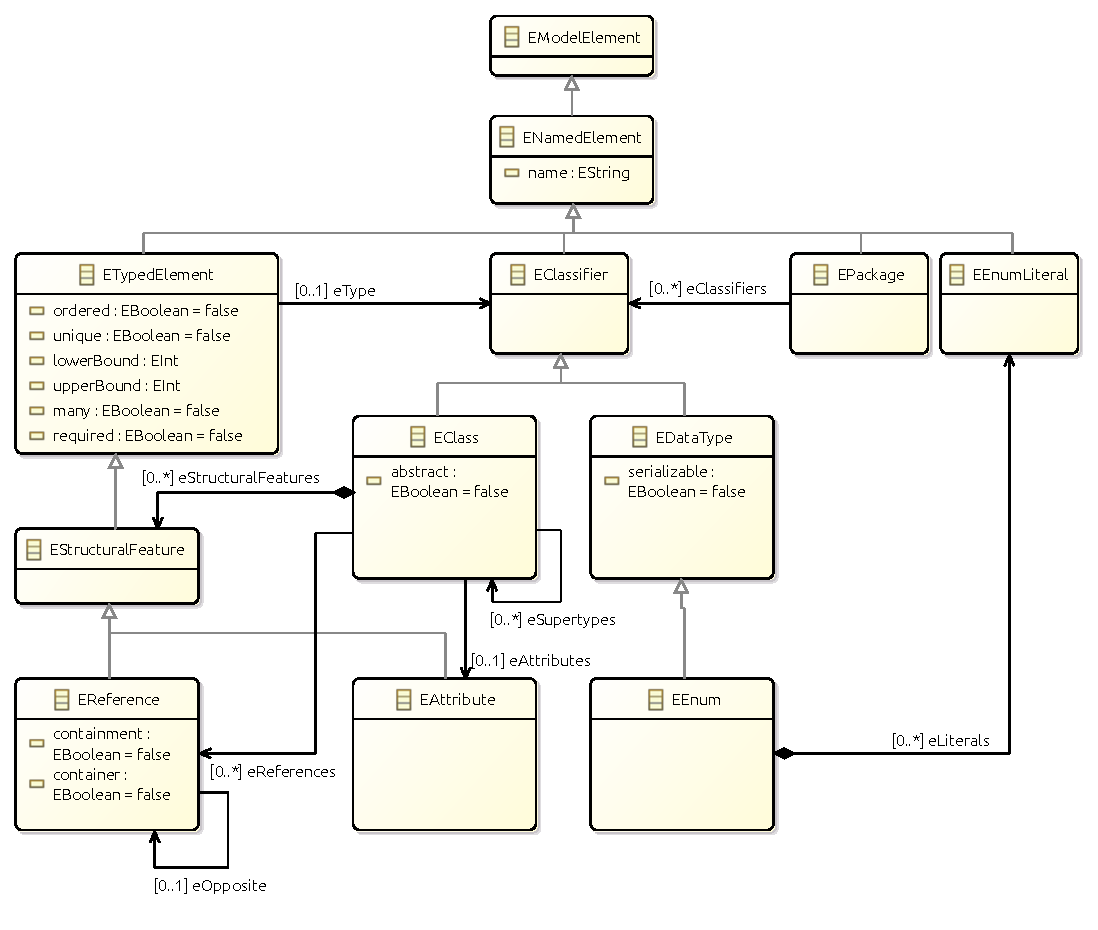
\includegraphics[width=\textwidth]{images/03_formalisations/02_ecore_formalisation/ecore.pdf}
    \caption{Simplified version of the Ecore metamodel}
    \label{fig:formalisations:ecore_formalisation:ecore}
\end{figure}

The Eclipse Modeling Framework (EMF) \cite{emf-gronback} is a modelling framework and code generation facility for building applications based on a structured model. It is quite popular in the field of Model-Driven Engineering because of its open-source nature. EMF offers support for creating, editing and translating models based on its metamodel Ecore \cite{bacvanski_graff_2005}. Models based on the Ecore metamodel are very comparable to UML class diagrams, but with properties specifically focused on software development. This focus makes models based on Ecore very suitable for object-oriented code generation as the structure of the model is already very similar to the class diagram of the corresponding application.

Because of the open-source nature of the Ecore metamodel and EMF, it has become increasingly popular for expressing domain models, creating editors for domain logic and code generation from domain models. However, EMF does not provide functionality for automated verification of its models out of the box. Different tools should be used to accomplish this task.

This thesis will focus on two levels of models based on the Ecore metamodel. The first level of models are models directly based on the Ecore metamodel, which will be called type models throughout this thesis. The second level of models are models based on a type model, and thus indirectly on the Ecore metamodel, and will be called instance models throughout this thesis. A simplified version of the Ecore metamodel \cite{emf_documentation_2015} with elements relevant to the formalisation is given in \cref{fig:formalisations:ecore_formalisation:ecore}.

\begin{figure}[H]
    \centering
    \begin{subfigure}{0.45\textwidth}
        \centering
        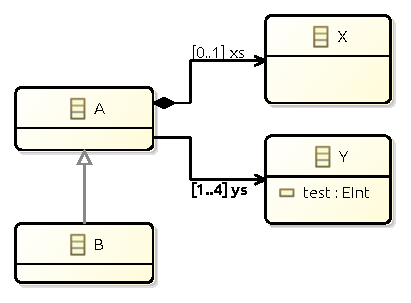
\includegraphics{images/01_introduction/type_model_intro.pdf}
        \caption{Type model}
        \label{fig:introduction:eclipse_modeling_framework:type_model}
    \end{subfigure}
    \begin{subfigure}{0.45\textwidth}
        \centering
        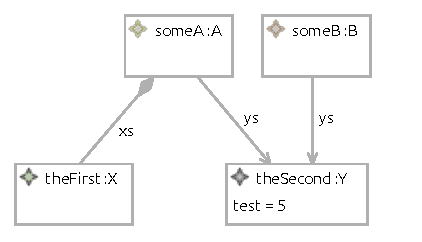
\includegraphics{images/01_introduction/instance_model_intro.pdf}
        \caption{Instance model}
        \label{fig:introduction:eclipse_modeling_framework:instance_model}
    \end{subfigure}
    \caption{Examples of different models in Ecore}
    \label{fig:introduction:eclipse_modeling_framework:ecore}
\end{figure}

\subsection{Type models}
\label{subsec:introduction:eclipse_modeling_framework:type_models}
A type model represents the first level of models based on the Ecore metamodel that will be used within this thesis. Since a type model is directly based on the Ecore metamodel, the metamodel of a type model is the Ecore metamodel. Since models based on the Ecore metamodel can best be understood as UML class diagrams, a type model can best be compared to a UML class diagram. \cref{fig:introduction:eclipse_modeling_framework:type_model} shows the visual notation of a type model in EMF's own visual notation. Familiar concepts from class diagrams can be found in this visualisation. First of all, the figure shows four class types, $\type{A}$, $\type{B}$, $\type{X}$ and $\type{Y}$. An example of inheritance of class types is shown, as class $\type{B}$ extends class $\type{A}$, so class $\type{B}$ is a subtype of class $\type{A}$. $\type{A}$ has two relations, named $\type{xs}$ and $\type{ys}$. Relation $\type{xs}$ is a relation to class $\type{X}$. Furthermore, the figure shows that $\type{xs}$ is a containment relation with a multiplicity of $0..1$. There is a second relation $\type{ys}$, which has a multiplicity of $1..4$. Finally, class $\type{Y}$ has an attribute named $\type{test}$, which represents an integer.

\subsection{Instance models}
\label{subsec:introduction:eclipse_modeling_framework:instance_models}
An instance model is the second level of models based on the Ecore metamodel that will be used in this thesis. An instance model is directly based on a type model. Therefore, the metamodel of an instance model is its corresponding type model. As a consequence, the metametamodel of an instance model is the Ecore metamodel. \cref{fig:introduction:eclipse_modeling_framework:instance_model} shows the visual notation of an instance model based on EMF's own notation, typed by the type model of \cref{fig:introduction:eclipse_modeling_framework:type_model}. The figure shows one instance of every class type. The instance of class $\type{A}$ has values for both the relations $\type{xs}$ and $\type{ys}$. The $\type{xs}$ relation references the instance of class $\type{X}$ and the $\type{ys}$ relation the instance of class $\type{Y}$. The instance of class $\type{B}$ only has a value for the relation $\type{ys}$, which references the instance of class $\type{Y}$. The instance of class $\type{Y}$ has a value set for the $\type{test}$ attribute, which is equal to integer $5$. Finally, all instances have a corresponding identifier, which is $someA$ for the instance of class $\type{A}$, $someB$ for the instance of class $\type{B}$, $theFirst$ for the instance of class $\type{X}$ and $theSecond$ for the instance of class $\type{Y}$.